\documentclass{beamer}
\usepackage[utf8]{inputenc}
\usepackage{lipsum}
\usepackage{xcolor}
\usepackage[T1]{fontenc}
\usepackage{parskip}
\usepackage{tabularx}
\usepackage{textgreek}

\usepackage{media9}
\usepackage{graphicx}
%\usepackage{fontspec}
\usepackage[roman]{parnotes}

\usepackage{utopia} %font utopia imported

\usepackage{array}
\newcolumntype{P}[1]{>{\centering\arraybackslash}p{#1}}

\usetheme{inrad}

\makeatletter
    \newenvironment{withoutheadline}{
        \setbeamertemplate{headline}[default]
        \def\beamer@entrycode{\vspace*{-\headheight}}
    }{}
\makeatother

\makeatletter
    \newenvironment{withoutfootline}{
        \setbeamertemplate{footline}[default]
        \def\beamer@entrycode{\vspace*{-\headheight}}
    }{}
\makeatother

\def\vfilll{\vskip 0pt plus 1filll minus 0pt }

\usepackage[style=authoryear,backend=bibtex8,doi=false,isbn=false,url=false,eprint=false]{biblatex}
\renewbibmacro{in:}{}
\AtEveryCitekey{%
    \clearfield{volume}%
    \clearfield{number}%
    \clearfield{title}%
    \clearfield{pages}}
\addbibresource{library.bib}

%------------------------------------------------------------
%This block of code defines the information to appear in the
%Title page
\title[Abstract Title] %optional
{This is the name of your presentation}

%\subtitle{An IMSA-branded Beamer template for SIR presentations}

\author[Authors] % (optional)
{\textbf{Author1\inst{1}\textsuperscript{,}\inst{2}}; Author2\inst{3}\textsuperscript{,}\inst{4}; Author3\inst{5}; author4\inst{2}}

\institute[] % (optional)
{
  \inst{1}%
  LIM44, Instituto e Departamento de Radiologia, Faculdade de Medicina, Universidade de Sao Paulo - Sao Paulo, Brazil; \hfill
  \inst{2}% \hfill
  Institution 2;
  \inst{3} \hfill
  Institution 3;
  \inst{4} \hfill
  Institution 4;
  \inst{5} \hfill
  Institution 5.
}

\date[Sao Paulo 2021] % (optional)
{Sao Paulo, April 13\textsuperscript{th}, 2021}



%End of title page configuration block
%------------------------------------------------------------
% Patch to move title block down
\usepackage{etoolbox}% http://ctan.org/pkg/etoolbox
%makeatletter
%  \newenvironment{settitle}{
%   \expandafter\patchcmd\csname beamer@@tmpl@title page\endcsname% <cmd>
%   {\vfill}% <search> 
%    {\vspace*{0.4in}}% <replace>
%    {}{}% <success><failure>
%    }{}
%\makeatother


%------------------------------------------------------------
%The next block of commands puts the table of contents at the 
%beginning of each section and highlights the current section:

%\AtBeginSection[]
%{
%  \begin{frame}
%    \frametitle{Table of Contents}
%    \tableofcontents[currentsection]
%  \end{frame}
%}
%------------------------------------------------------------


\begin{document}

% Title Page

\begin{withoutheadline}
\begin{withoutfootline}
%\begin{settitle}
  \usebackgroundtemplate{
\includegraphics[width=\paperwidth]{titlebackground.png}}
  %\vspace*{0.1in}
  \begin{frame}[plain]
    \vfill
    \vfill
    %\vfilll
    \vspace*{0.4in}
    \titlepage
    %\vfilll
    \usebeamerfont{institute} \centering \textcolor{black}{Contact: \url{email@usp.br}}
    %{Contact: \url{andre.paschoal@usp.br}}
  \end{frame}
%\end{settitle}
\end{withoutfootline}
\end{withoutheadline}
% use points template from now on
%\usebackgroundtemplate{
\includegraphics[width=\paperwidth]{pointbackground.png}}

%---------------------------------------------------------
%This block of code is for the table of contents after
%the title page
%---------------------------------------------------------

\section[Intro]{Introduction}

%---------------------------------------------------------
%Changing visibwility of the text

\begin{frame}
    \frametitle{Title of your slide}
    \begin{itemize}
        \item \small{Example of text in an item bullets.}
    \end{itemize}
    \vfill
    %\centering

    \footnotetext[1]{\fullcite{Louis2016}} %To add your reference, copy your library (.bib file) to the presentation folder.
\end{frame}

%---------------------------------------------------------


%---------------------------------------------------------
%Example of the \pause command
\begin{frame}
    \frametitle{Example of pause command}
    In this slide \pause
    
    the text will be partially visible \pause
    
    And finally everything will be there
\end{frame}
%---------------------------------------------------------

\section[Methods]{Methods}

%---------------------------------------------------------
%Highlighting text
\begin{frame}
    \frametitle{Methods}
    \begin{itemize}
        \item Data acquisition
    \end{itemize}
    \begin{table}
    %\caption{CNS pathologies involving BBB dysfunction.}
    %\label{tab:tabela_1}
        \resizebox{\textheight}{!}{% Resize table to fit within \linewidth horizontally
        \begin{tabular}{|P{0.3\textwidth}|P{0.3\textwidth}|P{0.3\textwidth}|P{0.3\textwidth}|}%{\linewidth}{l|X}
            \hline % Linha superior
            Text & Text & Text & Text mm\textsuperscript{2} \\ \hline % Linha do meio 
            Text & Text & Text & Text \\ \hline
            Text & Text & Text & Text \\ \hline
            Text & Text & Text & Text \\ \hline
            \multicolumn{4}{|c|}{Example of multi columns merged!!!} \\ \hline
            %\\\bottomrule % Linha inferior
        \end{tabular}}
    \end{table}
        %Adapted from \cite{Abbott2010}
        \vfill
        \begin{columns}
        \column{0.6\textwidth}
        \begin{itemize}
            \item Example of adding two columns format to the slide
            \begin{itemize}
                \item Major item 1: 
                \begin{itemize}
                    \item sub-item1;
                    \item sub-item2;
                    \item sub-item3;
                    \item sub-item4;
                    \item sub-item5.
                \end{itemize}  
            \end{itemize}
        \end{itemize}

        \column{0.4\textwidth}
        \begin{itemize}
            \item Text for collumn 2; 
            \parnote[\(\dagger\)]{\label{note:dagger}Example of footnote} for MATLAB.
            \item Another item.
        \end{itemize}
        
        
    \end{columns}
    \parnotes

\end{frame}
%---------------------------------------------------------

\section[Cap1]{Results \& Discussion}

%---------------------------------------------------------
%Two columns
\begin{frame}
\frametitle{Title for results slide}

%\begin{figure}[!htb]
    %\centering
    %\includegraphics[width=\linewidth,height=0.85\textheight,keepaspectratio]{Figures/figure.png}
    %\label{justalabel}
%\end{figure}
\end{frame}

\begin{frame}
    \frametitle{Discussion}
    \begin{itemize}
        \item item1;
        \item item2;
        \item item3;
        \item item4;
        \item item5.
    \end{itemize}
\end{frame}



\begin{frame}
    \frametitle{Example of adding multiple figures to the slide}
    \begin{figure}
        \begin{minipage}{0.65\textwidth}
            \centering
            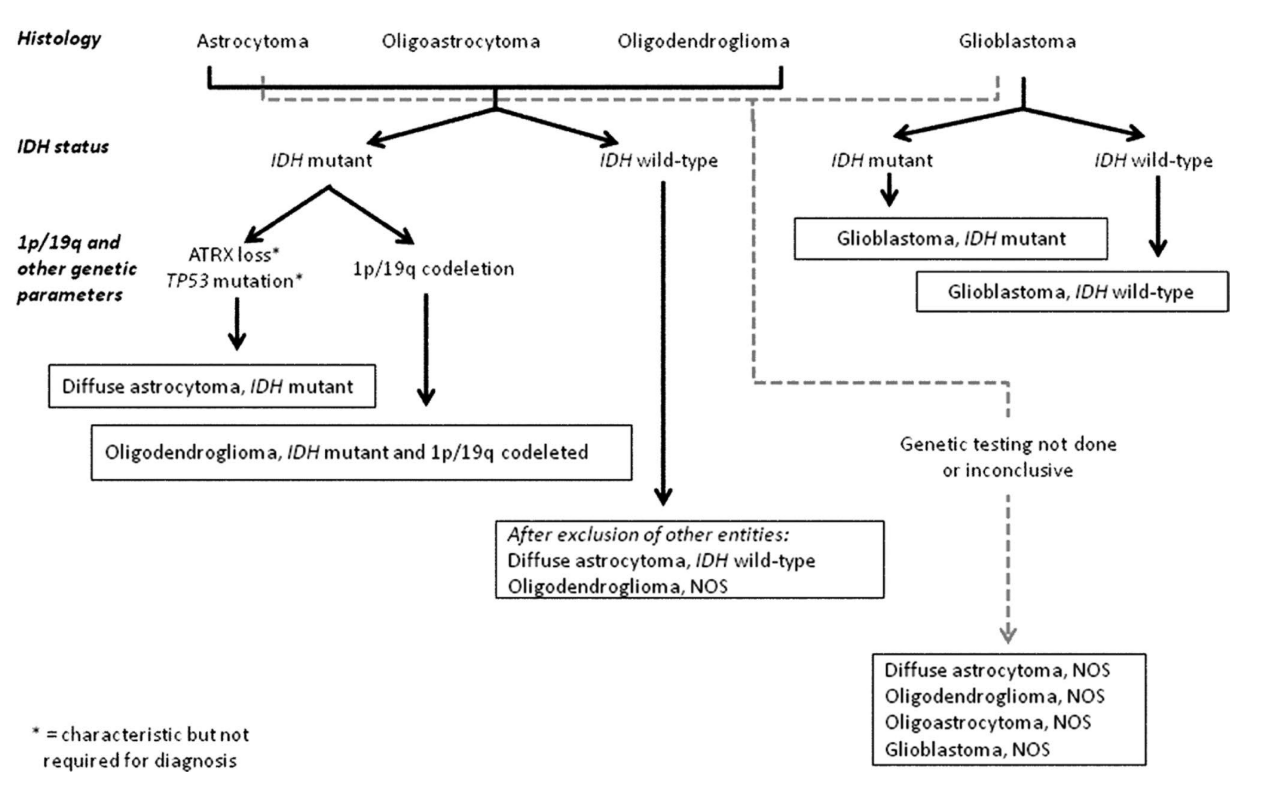
\includegraphics[width=\linewidth,height=0.4\textheight,keepaspectratio]{Figures/gliomaHist.png}
            %\caption{Exemplo de figura embutida no texto}
            \label{fig1}
        \end{minipage}\hfill
         \begin{minipage}{0.35\textwidth}
            \centering
            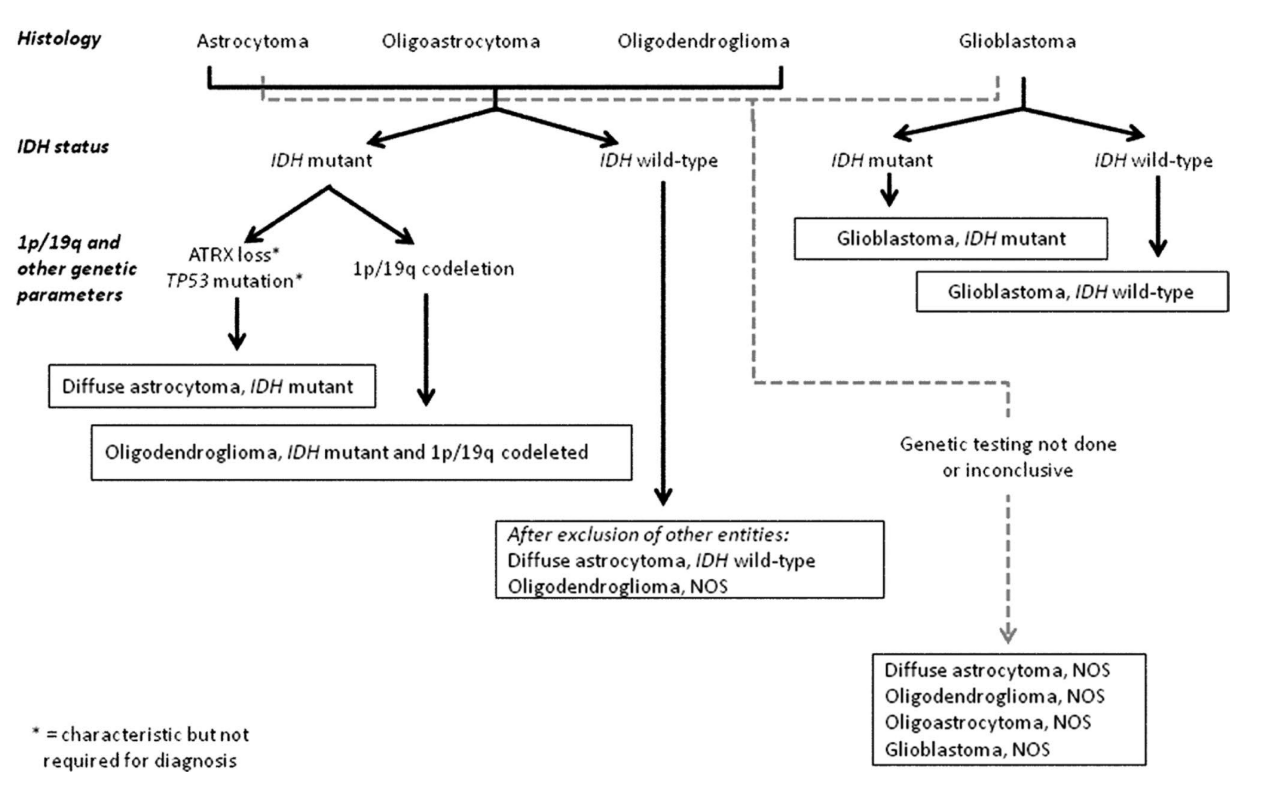
\includegraphics[width=\linewidth,height=0.4\textheight,keepaspectratio]{Figures/gliomaHist.png}
            %\caption{Exemplo de figura embutida no texto}
            \label{fig2}
        \end{minipage}
    \end{figure}
\end{frame}

%---------------------------------------------------------

\section[Conclusions]{Conclusions}

%---------------------------------------------------------

\begin{frame}
    \frametitle{Conclusions}
    \begin{block}{\centering \textbf{Take Home Message 1}}
        \centering \small{Key message 1.}
    \end{block}
    
    \begin{block}{\centering \textbf{Take Home Message 2}}
        \centering 
        \begin{itemize}
            \item \small{Item 1} 
            \item \small{Item 2}
        \end{itemize}
    \end{block}
     
\end{frame}

\begin{frame}
    \frametitle{Aknowledgements}
    \begin{figure}
        \begin{minipage}{0.6\textwidth}
            \centering
            \huge{\textbf{Thank you!}}
        \end{minipage}\hfill
        \begin{minipage}{0.4\textwidth}
            \centering
            \begin{minipage}{0.35\textheight}
                
\includegraphics[width=\linewidth,height=1\textheight,keepaspectratio]{Figures/fapesp.png}                
            \end{minipage}
            \begin{minipage}{0.35\textheight}
                
\includegraphics[width=\linewidth,height=1\textheight,keepaspectratio]{Figures/cnpq.png}
            \end{minipage}
            \begin{minipage}{0.35\textheight}
                
\includegraphics[width=\linewidth,height=1\textheight,keepaspectratio]{InradFrametitle.png}
            \end{minipage}
        \end{minipage}
    \end{figure}
\end{frame}


\end{document}